\documentclass{llncs}

\usepackage[utf8]{inputenc}
\usepackage[T1]{fontenc}
\usepackage[noadjust,nosort]{cite}
\usepackage{amsmath}
\usepackage{amsfonts}
\usepackage{amssymb}
%\usepackage{MnSymbol}
%\usepackage{thmtools}
%\usepackage{thm-restate}
\usepackage{booktabs}
\usepackage{figlatex}
\usepackage{xcolor}
\usepackage{setspace}
\usepackage{xspace}
\usepackage[super]{nth}
\usepackage{multicol}
\usepackage{microtype}
\usepackage{wrapfig}
\usepackage{graphicx}
\usepackage{subfig}
\usepackage[center,width=152mm,height=235mm]{crop}
%\usepackage[pagewise,switch]{lineno} % switch, modulo, pagewise
\usepackage{hyperref}
%\usepackage[linesnumbered,lined,noend,ruled]{algorithm2e}
\usepackage[lined,noend,ruled]{algorithm2e}
\usepackage[capitalise,english,nameinlink]{cleveref} % load after algorithm2e and hyperref

\hypersetup{
  bookmarksdepth=2,
  bookmarksnumbered=true,
  bookmarksopen=true,
  bookmarksopenlevel=2,
  colorlinks=true,
  linktocpage=true,
  breaklinks=true,
  pageanchor=true,
  allcolors=[rgb]{0.6,0.0,0.0},
  pdftitle={DPU's data structures and algorithms},
  pdfauthor={Huyen N.T.T, César Rodríguez}
}

%\newcommand\comp {\mathfrak{c}}
%\newcommand\cycles[1]  {\mathsf{Cycles}{(#1)}}
%\newcommand\extn {\mathcal{X}}
%\newcommand\lchist[2]  {{ {#1}\langle#2\rangle }}
%\newcommand\lonepref   {\ppref^1_{N}}
%\newcommand\lpg     {\leadsto_\config}
%\newcommand\lstruc  {\mathcal{L}}
%\newcommand\ltwopref   {\ppref^2_{N}}
%\newcommand\maxspoilers[1]{t^{\spoils}_{#1}}
%\newcommand\move[1] {\stackrel{#1}{\longrightarrow }}
%\newcommand\myleq   \le
%\newcommand\nat     {\mathrm{I\!N}}
%\newcommand\node[1] {\mathit{#1}}
\newcommand\pac      {\mathrel{\nearrow\!\!\!\!\!\nearrow}}
\newcommand\rd       \propto
%\newcommand\spoils  {\dagger}

% relations
%\newcommand\reveals  {\mathrel{\triangleright}}
%\newcommand\ac       {\mathrel{\nearrow}}
\newcommand\aco      {\mathrel{/\!\!/}}
\newcommand\cfl      {\mathrel{\#}}
\newcommand\icfl[1][]{\mathrel{\#^i_{#1}}}
\newcommand\co       {\mathrel{\parallel}}
\newcommand\indep    {\mathrel{\meddiamond}}
\newcommand\depen    {\mathrel{\diamondtimes}}
\newcommand\eqdef    {\mathrel{:=}}
\newcommand\evolves  {\mathrel{\sqsubseteq}}
\newcommand\evstrict {\mathrel{\sqsubset}}
\newcommand\ispref   {\mathrel{\trianglelefteq}}
\newcommand\icause   {\mathrel{<_i}}
\newcommand\ifft     {\mathrel{\text{ iff }}}
\newcommand\nco      {\mathrel{\not\!\!\;\,\co}}
\newcommand\fire[1]  {\mathrel{\raisebox{-1.1pt}{$\xrightarrow{#1}$}}}

\newcommand\extreveals  {\mathbin{-\hspace{-2.5mm}-\hspace{-2.0mm}\reveals}}

% operators
\newcommand\iscutoff[1] {\mathop{\mathsf{cutoff}} (#1)}
\newcommand\union[1]    {\mathop{\mathit{union}} (#1)}
\newcommand\merge[1]    {\mathop{\mathfrak{Merge}} (#1)}
\newcommand\od[1]       {\mathop{\mathrm{od}} (#1)}
\newcommand\amo[1]      {\mathop{\textsf{AMO}} (#1)}
\newcommand\acyclic[1]  {\mathop{\textsf{ACY}} (#1)}
\newcommand\bigo[1]     {\mathop{\mathcal{O}} (#1)}
\newcommand\progloop[1] {\mathop{\mathit{ploop}} (#1)}
\newcommand\allhist[1]  {\mathop{\mathit{Hist}} (#1)}
\newcommand\compt[1]    {\mathop{\mathit{compat}} (#1)}
\newcommand\conc[1]     {\mathop{\mathit{conc}} (#1)}
\newcommand\conf[1]     {\mathop{\mathit{conf}} (#1)}
\newcommand\cut[1]      {\mathop{\mathit{cut}} (#1)}
\newcommand\explain[1]  {\mathop{\mathit{expl}} (#1)}
\newcommand\lpo[1]      {\mathop{\mathit{lpo}} (#1)}
\newcommand\marking[1]  {\mathop{\mathit{mark}} (#1)}
\newcommand\obser[1]    {\mathop{\mathit{obs}} (#1)}
\newcommand\peel[2]     {\mathop{\mathit{peel}}_{#2} (#1)}
\newcommand\peelast[1]  {\mathop{\mathit{peelmax}} (#1)}
\newcommand\reach[1]    {\mathop{\mathit{reach}} (#1)}
\newcommand\runs[1]     {\mathop{\mathit{runs}} (#1)}
\newcommand\sfp[1]      {\mathop{\mathit{pred}} (#1)}
\newcommand\spoilers[1] {\mathop{\mathit{spoilers}} (#1)}
\newcommand\state[1]    {\mathop{\mathit{state}} (#1)}
\newcommand\succexpl[1] {\mathop{\mathit{succexpl}} (#1)}
\newcommand\trim[2]     {\mathop{\mathit{trim}_{#2}} (#1)}
\newcommand\trimast[1]  {\mathop{\mathit{trimmax}} (#1)}
\newcommand\depth[1]    {\mathop{\mathit{depth}} (#1)}
\newcommand\pe[1]       {\mathop{\mathit{pe}} (#1)}
\newcommand\inter[1]    {\mathop{\mathit{inter}} (#1)}
\newcommand\proc[1]     {\mathop{\mathit{proc}} (#1)}
\newcommand\enabl[1]    {\mathop{\mathit{enabl}} (#1)}
\newcommand\en[1]       {\mathop{\mathit{en}} (#1)}
\newcommand\ex[1]       {\mathop{\mathit{ex}} (#1)}
\newcommand\cex[1]      {\mathop{\mathit{cex}} (#1)}
\newcommand\fcfl[1]     {\mathop{\mathit{\#}} (#1)}
\newcommand\ficfl[2][]  {\mathop{\mathit{\#^i_{#1} }} (#2)}
\newcommand\forml[1]    {\mathcal{L} (#1)}

\newcommand\mult[1]     {\mathbf{#1}}
\newcommand\sem[1]      {\mathrm{[\![{#1}]\!]}}
\newcommand\hist[2]     {{ {#1}[\![#2]\!] }}
\newcommand\cont[1]     {\underline{#1}}
\newcommand\post[1]     {#1^\bullet}
\newcommand\pre[1]      {{}^\bullet#1}
\newcommand\support[1]  {\bar{#1}}
\newcommand\causes[1]   {\left \lceil #1 \right \rceil}
\newcommand\future[1]   {\left \lfloor #1 \right \rfloor}

\newcommand\FIXME[1]    {\textcolor{red}{\texttt{FIXME: #1}} }
\newcommand\anc[1]      {{#1}^\uparrow}
\newcommand\eenr        {\mathcal{E}}
\newcommand\enr[1]      {\mathcal{E}_{#1}}
%\newcommand\pes         {\mathcal{E}}
\newcommand\les         {\mathcal{E}}
\newcommand\unf[1]      {\mathcal{U}_{#1}}
\newcommand\unr[1]      {\mathcal{M}_{#1}}
\newcommand\var[1]      {\mathsf{#1}}
\newcommand\mer[1]      {\mathcal{Q}_{#1}}
\newcommand\hst[1]      {\mathcal{H}_{#1}}
\newcommand\trunc[1]    {\mathcal{T}_{#1}}
\newcommand\htrunc[1]   {\widehat{\mathcal{T}}_{#1}}
\newcommand\pref[1]     {\mathcal{P}_{#1}}
\newcommand\precpref[1] {\mathcal{P}^\prec_{#1}}
\newcommand\trace[1]    {\mathcal{T}_{#1}}
\newcommand\dgraph[1]   {\mathcal{D}_{#1}}
\newcommand\intsem[1]   {\mathcal{S}_{#1}}
\newcommand\cutoffs     {\mathcal{K}}

% abbreviations
\newcommand\precutoff{\text{$\prec$-cutoff}}
\newcommand\phiasym  {\phi_\ppref^\text{asym}}
\newcommand\phicausal{\phi_\ppref^\text{causal}}
\newcommand\phiconf  {\phi_\ppref^\text{conf}}
\newcommand\phidead  {\phi_\ppref^\text{dead}}
\newcommand\phidis   {\phi_\ppref^\text{dis}}
\newcommand\phimark  {\phi_\ppref^{\text{mark},M}}
\newcommand\phicov   {\phi_\ppref^{\text{cov},M}}
\newcommand\phip     {\phi_\ppref}
\newcommand\phisym   {\phi_\ppref^\text{sym}}

\newcommand\mphimark {\gamma_\qpref^{\text{mark},M}}
\newcommand\mphicon  {\gamma_\qpref^{\text{con},M}}
\newcommand\mphiaux  {\gamma_\qpref^\text{aux}}
\newcommand\mphiflow {\gamma_\qpref^\text{flow}}
\newcommand\mphiasym {\gamma_\qpref^\text{asym}}
\newcommand\mphicov  {\gamma_\qpref^{\text{cov},M}}
\newcommand\mphigap  {\gamma_\qpref^\text{no-gap}}
\newcommand\mphipath {\gamma_\qpref^\text{path}}

\newcommand\mphiconf {\gamma_\qpref^\text{conf}}
\newcommand\mphidis  {\gamma_\qpref^\text{dis}}
\newcommand\mphip    {\gamma_\qpref}


\newcommand\mcitomp  {\textsc{Mci2mp}\@\xspace}
\newcommand\minisat  {\textsc{Minisat}\@\xspace}
\newcommand\mole     {\textsc{Mole}\@\xspace}
\newcommand\prcompress{\textsc{PRCompress}\@\xspace}
\newcommand\clp      {\textsc{Clp}\@\xspace}
\newcommand\cmerge   {\textsc{Cmerge}\@\xspace}
\newcommand\cunf     {\textsc{Cunf}\@\xspace}
\newcommand\poet     {\textsc{Poet}\@\xspace}
\newcommand\nidhugg  {\textsc{Nidhugg}\@\xspace}
\newcommand\cosyverif{\textsc{Cosyverif}\@\xspace}
\newcommand\coloane  {\textsc{Coloane}\@\xspace}
\newcommand\tapaal   {\textsc{Tapaal}\@\xspace}
\newcommand\cunft    {Cunf~Toolset}
\newcommand\cna      {\textsc{Cna}\@\xspace}
\newcommand\punf     {\textsc{Punf}\@\xspace}
\newcommand\salpha   {\ppref_\alpha}
\newcommand\spcutoff {\text{sp-cutoff}}
\newcommand\id       {\textit{id}}
\newcommand\ep       {EP}
\newcommand\dr       {Dr.\@\xspace}
\newcommand\mr       {Mr.\@\xspace}
\newcommand\prof     {Prof.\@\xspace}

\newcommand\uunf     {\mathcal{U}}
\newcommand\ppref    {\mathcal{P}}
\newcommand\qpref    {\mathcal{Q}}
\newcommand\con      {\mathcal{C}}
\newcommand\N        {\mathbb{N}}
\newcommand\Q        {\mathbb{Q}}
\newcommand\R        {\mathbb{R}}
\newcommand\obs      {\mathbb{O}}
\newcommand\hhat     {\widehat h}
\newcommand\ehat     {\widehat e}
\newcommand\chat     {\widehat c}
\newcommand\conhat   {\widehat \con}
\newcommand\Hhat     {\widehat H}
\newcommand\Ehat     {\widehat E}
\newcommand\Bhat     {\widehat B}
\newcommand\cgen     {\var{c_{\text{gen}} }}
\newcommand\cpgen    {\var{c'_{\text{gen}} }}
\newcommand\ccon     {\var{c_{\text{con}} }}
\newcommand\ccut     {\var{c_{\text{cut}} }}

\newcommand\pp       {pp.\@\xspace}
\newcommand\viz      {viz.\@\xspace}
\newcommand\vs       {vs.\@\xspace}
\newcommand\wlogg    {w.l.o.g.\xspace}
\newcommand\aka      {a.k.a.\xspace}
\newcommand\wrt      {w.r.t.\@\xspace}
\newcommand\cf       {cf.\@\xspace}
\newcommand\Wlog     {W.l.o.g.\xspace}
\newcommand\al       {al.\@\xspace}
\newcommand\eg       {e.g.\@\xspace}
\newcommand\etc      {etc.\@\xspace}
\newcommand\ie       {i.e.\@\xspace}
\newcommand\naive    {na{\"\i}ve\xspace}
%\newcommand\st      {s.t.\@\xspace}
\newcommand\resp     {resp.\@\xspace}
\newcommand\nr       {nr.\@\xspace}
\newcommand\avg      {avg.\@\xspace}

% miscellaneous
\newcommand\cod[1]   {\texttt{#1}}
\newcommand\tup[1]   {\langle#1\rangle}
\newcommand\set[1]   {{\{ #1 \mathclose \}}}
\newcommand\eqtag[1] {\hfill{} \refstepcounter{equation} \label{#1} (\arabic{equation})}

%\newtheorem{cor} {Corollary}
%\newtheorem{defn}   {Definition}
%\newtheorem{lemma}  {Lemma}
%\newtheorem{proposition}{Proposition}
%\newtheorem{remark} {Remark}
%\newtheorem{theorem}   {Theorem}

%\renewcommand{\algorithmicensure}{\textbf{Output}:}
%\renewcommand{\algorithmicrequire}{\textbf{Input}:}
%\renewcommand{\labelitemi}{\textbf{--}}
%\renewcommand{\labelitemi}{{\footnotesize $\bullet$}}

% e  equation
% d  def
% f  figure
% l  lemma, line
% s  section
% r  remark
% p  proposition
% t  theorem
% c  corollary
% b  table
% a  algorithm
% x  appendix
% h  chapter
% n  footnote
% m  example

% for standard names
\crefname{equation}{}{}
\crefname{proposition}{Prop.}{Props.}
\Crefname{proposition}{Proposition}{Propsitions}
\crefname{section}{\S}{\S\S}
\Crefname{section}{Section}{Sections}
\crefname{page}{p.}{pp.}
\Crefname{page}{Page}{Pages}
\crefname{chapter}{Ch.}{Ch.}
\Crefname{chapter}{Chapter}{Chapters}
\crefname{remark}{Rmk.}{Rmks.}
\Crefname{remark}{Remark}{Remarks}
\crefname{appendix}{App.}{App.}
\Crefname{appendix}{Appendix}{Appendix}
\crefname{algorithm}{Alg.}{Alg.}
\Crefname{algorithm}{Algorithm}{Algorithms}
%\crefname{algocf}{algorithm}{algorithm}
%\Crefname{algocf}{Algorithm}{Algorithm}
\crefname{line}{line}{line}
\Crefname{line}{Line}{Line}

% for LIPICs
\crefname{theo}{Theorem}{Theorems}
\crefname{lem}{Lemma}{Lemmas}
\crefname{cor}{Corollary}{Corollaries}
\crefname{prop}{Prop.}{Props.}
\crefname{defn}{Def.}{Defs.}
\Crefname{defn}{Definition}{Definitions}
\crefname{exampl}{Example}{Examples}
\crefname{rmk}{Remark}{Remarks}

%\crefname{AlgoLine}{algorithm}{algorithm}




\title{DPU's Data Structures and Algorithms}
%\author{Huyen Nguyen \and C\'esar Rodr\'{\i}guez}
\author{TBD}
\institute{Université Paris 13, Sorbonne Paris Cité, LIPN, CNRS, France}

\begin{document}

\maketitle

\begin{abstract}
TBD
\end{abstract}

\section{Execution Model}
\label{s:model}

Relevant classes:
\verb!Machine!,
\verb!Process!,
\verb!Trans!,
\verb!State!

Transition types :
\begin{itemize}
\item
  \verb!RD! Represents a transition that performs a certain amount of
  local (independent) work plus a single read operation on some global variable.
\item
  \verb!WR! Represents a transition that performs a certain amount of
  local (independent) work plus a single write operation on some global variable.
\item
  \verb!LOC! Represents a transition that only performs local (independent)
  operations.
\item
  \verb!SYN! Represents a synchronization operation, intended to model a
  lock or unlock operation on a mutex.
\end{itemize}

\subsection{Data Structure}

FIXME

\section{Unfolding}

Relevant classes:
\verb!Unfolding!.

\subsection{Data Structure}

A vector of \verb!Event!s, a pointer to the bottom event, and a reference
to the \verb!Machine!.

\section{Event}
Relevant classes:
\verb!Event!.

Events represent the occurrence of transitions.
They store pointers to all their immediate causal predecessors (ICPs), and some of
the immediate causal successors (ICSs).
The number of ICPs is determined by the type of the transition they
represent:

\begin{itemize}
\item \verb!LOC! events: 1 predecessor (process)
\item \verb!SYN! events: 2 predecessors (process, last \verb!SYN! on same variable)
\item \verb!RD!  events: 2 predecessor (process + last \verb!RD! or
	\verb!WR! operation on the same variable)
\item \verb!WR!  events: 1 predecessor (process) + one predecessor per
	process (last \verb!RD! or \verb!WR! operation on that process)
\end{itemize}

The immediate causal successors of one event are determined by those events
for which the event is an immediate causal predecessor. Some of the causal
successors are stored in the \verb!Event! class, but not all.

FIXME -- some of these events are only causal predecessors or successors,
not necessarily immediate predecessors or successors.

\subsection{Data Structure}
The members of the class \verb!Event! that are relevant on each instance of
the class depend on the type of the transition represented by the event.

All kinds of events store:
\begin{itemize}
\item
  \verb!trans!: a pointer to the transition it represents.
\item
  \verb!localvars!: vector (\verb!std::vector!) of \verb!uint32_t! values
  containing the value of the variables whose addresses are strored in
  \verb!this->trans->localvars!.
\item
  \verb!pre_proc!: (ICP) a pointer to the last event in the same thread.
\item
  \verb!post_proc!: (ICSs) a vector (\verb!std::vector!) of pointers to
  the next events in the same thread.
\end{itemize}
%
For \verb!SYN! events :
\begin{itemize}
\item
  \verb!pre_mem!: (ICP) pointer to the last \verb!SYN! event on the same
  variable, possibly performed by the same thread or another thread.
  Recall that \verb!SYN! operations on the same variable induce a tree when
  regarded unfolding-wise, and a total order (a branch of that tree) when
  the attention is reduced to an arbitrary configuration.
  In this regard, \verb!pre_mem! is a pointer to the node's parent in that
  tree.
\item
  \verb!post_mem!: (ICSs) vector (\verb!std::vector!) of pointers to
  the immediate next \verb!SYN! operations on the same variable, in this or
  another thread. These are the children of the aforementionned
  unfolding-wise tree.
\item
  \verb!val!: the value written by this event to the variable \verb!trans->var!
\end{itemize}
%
For \verb!RD! events :
\begin{itemize}
\item
  \verb!pre_mem!: (ICP) pointer to the last \verb!RD! or \verb!WR! event of
  the same thread. Observe that we do not store anything in the
  \verb!post_mem! vector.
\end{itemize}
%
Finally, for \verb!WR! events :
\begin{itemize}
\item
  \verb!pre_mem!: (causal predecessor) pointer to the last event
  representing a \verb!WR! operation performed on the same variable.
  Recall that \verb!WR! operations on the same variable induce a tree when
  regarded unfolding-wise, and a total order (a branch of that tree) when
  the attention is reduced to an arbitrary configuration.
  In this regard, \verb!pre_mem! is a pointer to the node's parent in that
  tree.
\item
	
  \verb!post_wr!: (causal WR successsor) vector (\verb!std::vector!) of
  pointers to the next \verb!WR! operations on the same variable, in this
  or another thread. These are the children of the aforementionned
  unfolding-wise tree.(need re-considered its existence)
\item
  \verb!post_mem!: (causal RD, SYN, WR immediate successors) a vector of vectors (\verb!std::vector<std::vecotr>!) of operations on the same variable in differents threads. 
	
\item
  \verb!pre_readers!: (immediate and not immediate causal predecessors)
  vector (\verb!std::vector!) of pointers to events (one per thread).
  The event pointed is the last \verb!RD! or \verb!WR! operation on the
  same variable performed in that thread.
\end{itemize}

FIXME - incomplete; look at my notes and fix


\subsection{Conflict between events}
To determine immediate conflict between two events $e$ and $e'$: 
\begin{itemize}
	\item
		One of them is a LOC, there is no conflict at all.
	\item
		If they have the same predecessor \verb!e.pre_proc = e'.pre_proc!, the look at their local configuration.
	\item
		If they are in different processes (have different \verb!pre_proc!), look at one event's \verb!parent! \verb!e.pre_mem! (watch out the case where its parent is $bottom$ - a special WR)
	\begin{itemize}
		\item
			\verb!parent! is RD or SYN: if we find $e'$ in its \verb!post_rws!, then they are in
			 conflict.
		\item
			\verb!parent! is WR: if we find $e$ and $e'$ in the same vector of \verb!e.post_mem!,
			 they are in conflict (e can be a WR, so it can appear in all vectors of 
			 \verb!e.post_mem!, not only the vector of its process)
	\end{itemize}
		
\end{itemize}

\section{Configuration}
Relevant classes:
\verb!Config!.

\subsection{Data Structure}

\begin{itemize}
\item
  \verb!state!: the state reached by the configuration (type \verb!ir::State!).
\item
  \verb!latest_proc!:
  a vector of pointers to events. The size of the vector is the number of
  processes. Conceptually this represents a function from the set of processes
  to the set of events, which gives, for every process, the (unique) causally
  maximal event of that process in the configuration.

\item
  \verb!latest_wr!
  a vector of pointers to events. Size: the number of variables of the system.
  Conceptually this represents a function from the set of variables
  to the set of events, which gives, for every variable, latest (causally
  maximal) event that wrote to the variable (that event must correspond to a
  \verb!SYN! or \verb!WR! transition).

\item
  \verb!latest_op!
  a vector of pointers to events. Size: the number of variables times number of
  processes.
  Conceptually this represents a function $f \colon P \times V \to C$,
  where $P$ is the set of processes, $V$ is the set of variables, and $C$ the
  set of events in the configuration.
  The event $f (p,v)$ is the latest (causally maximal) operation that process
  $p$ performed on variable $v$ (it will correspond to a \verb!SYN!, \verb!WR!,
  or \verb!RD! transition).
\end{itemize}

\subsection{Enabled Events}

\begin{itemize}
\item
  Enumerate all transitions enabled at the \verb!state!
\item
  Using the members variables it is easy to construct new events.
\end{itemize}

\subsection{Conflicting Extensions}


Let $M$ be the input program model.
Let $\unf M \eqdef \tup{E,<,\cfl,h}$ be the unfolding of $M$.
Let $t$ be a transition of $M$ and $C \subseteq E$ a configuration of $\unf M$.
See \cite{RSSK15} for a formal definition.

In the sequel we give an algorithm to compute the \emph{conflicting extensions}
of~$C$, defined as
$
\cex C \eqdef
\set{e \in \ex C \colon \exists e' \in C,\, e \icfl{} e'},
$
where the \emph{extensions} of~$C$, written $\ex C$,
are all those events outside~$C$ whose causes are included in~$C$.
Formally,
$
\ex C \eqdef
\set{e \in E \colon e \notin C \land \causes e \subseteq C}
$, where
$\causes e \eqdef \set{e' \in E \colon e' < e}$.
Again, see \cite{RSSK15long} to gain intuition about the necessity and motivation
behind these definitions.

Assume we are given a configuration $C$.
We want to compute all events in $\cex C$.
Let \verb!t! be a transition of $M$.
For each type of transition we give a different algorithm that computes all
events $e \in E$ such that $h(e) = t$:
\begin{itemize}
\item Apply \cref{a:cex_rd} if $t$ is \verb!RD! transition.
\item Apply \cref{a:cex_syn} if $t$ is \verb!SYN! transition.
\item Apply \cref{a:cex_wr} if $t$ is \verb!WR! transition.
\item If $t$ is a \verb!LOC! transition, then there is no conflicting extension
$e \in \cex C$ such that $h(e) = t$.
\end{itemize}

\begin{theorem}[Conflicting extensions]
Let $M$ be the model of a program as described in \cref{s:model}.
Let $C$ be an arbitrary configuration of $\unf M$.
Then the algorithm above computes exactly the set of events $\cex C$.
\end{theorem}
\begin{proof}
TBD
\end{proof}

\Cref{a:cex_wr} is slightly more complex than the algorithms for read and
synchronization transitions, and requires the following additional definitions.

Let $A$ be a set.
A \emph{comb} over~$A$ of size $n \in \N$ is an $n$-tuple
$c \eqdef \tup{s_1, \ldots, s_n}$ of sequences $s_i \in A^*$
over~$A$.
Each sequence $s_i$ of the $n$-tuple is called a \emph{spike}.
Given a comb $c$ of size~$n$,
a \emph{combination} of $c$ is any $n$-tuple $\tup{a_1, \ldots, a_n} \in A^n$
such that $a_i \in A$ is one of the elements of the sequence $s_i \in A^*$, for
$i \in \set{1, \ldots, n}$.

Let $e \in E$ be a \verb!WR! event in $\unf M$.
Let $\set{e_1, \ldots, e_n}$ be the set of \verb!pre_readers! of~$e$.
We define the \emph{comb associated to $e$} as the only comb
$\tup{s_1, \ldots s_n}$ of size~$n$ over~$E$ defined as follows:
\begin{itemize}
\item
  Sequence $s_i \in E^*$ is formed by all \verb!RD! events and the only
  \verb!WR! event that can be found by recursively exploring the pointer
  \verb!pre_mem! starting from event~$e_i$. The last event to include in the
  sequence is the first event of type \verb!WR! found during the exploration of
  the list.
\end{itemize}


\begin{algorithm}
\noindent
For each event $e \in C$ such that \verb!e->trans == t!, repeat the following:
\begin{enumerate}
\item Set \verb!ep = e->pre_proc!
\item Set \verb!em = e->pre_mem!
\item If $\verb!em! < \verb!ep!$, then goto End.
\item If \verb!em! is \verb!RD!, then set \verb!em = em->pre_mem!
\item If not, it must necessarily be \verb!WR!; then set \verb!em = em->pre_readers[t->proc]!
\item (Warning: check for the bottom event in previous calculation)
\item
  Create (or retrieve) an event \verb!ex! such that
  \begin{itemize}
  \item \verb!ex->trans = t!,
  \item \verb!ex->pre_proc = ep!,
  \item \verb!ex->pre_mem = em!,
  \end{itemize}
  
\item Check if \verb!ex! is enabled at the new local configuration
\item Event \verb!ex! is in $\cex C$
\item Goto 4.
\item End.
\end{enumerate}
\caption{Conflicting extesions associated to \texttt{RD} transitions.}
\label{a:cex_rd}
\end{algorithm}

\begin{algorithm}
\noindent
For each event $e \in C$ such that \verb!e->trans == t!, repeat the following:
\begin{enumerate}
\item Set \verb!ep = e->pre_proc!
\item Set \verb!em = e->pre_mem!
\item If $\verb!em! < \verb!ep!$, then goto End.
\item Set \verb!em = em->pre_mem!
\item (Warning: check for the bottom event in previous calculation)
\item
  Create (or retrieve) an event \verb!ex! such that
  \begin{itemize}
  \item \verb!ex->trans = t!,
  \item \verb!ex->pre_proc = ep!,
  \item \verb!ex->pre_mem = em!,
  \end{itemize}
\item Event \verb!ex! is in $\cex C$
\item Goto 3.
\item End.
\end{enumerate}

\caption{Conflicting extesions associated to \texttt{SYN} transitions.}
\label{a:cex_syn}
\end{algorithm}

\begin{algorithm}
\noindent
For each event $e \in C$ such that \verb!e->trans == t!, repeat the following:
\begin{enumerate}
\item Set \verb!ep = e->pre_proc!
\item Set \verb!ew = e!
\item
  Let $M$ be the set of maximal events in $[e_p]$ that read or write variable
  \verb!t->var! ($M$ will either be a singleton with only \verb!WR! event or
  will contain exactly one \verb!RD! or \verb!WR! event per process)
\item If $\verb!ew! < \verb!ep!$, then goto End.
\item Let $c \eqdef \tup{s_1, \ldots, s_n}$ be the comb associated to \verb!ew!
\item
  Enumerate all combinations $\tup{e_1, \ldots, e_n}$ of $c$.
  For any of them, do:
  \begin{enumerate}
  \item
    If $\tup{e_1, \ldots, e_n} = \verb!e->pre_readers!$, then discard and take
    next one.
  \item
    If any event in $\set{e_1, \ldots, e_n}$ is a causal predecessor of some event in
    $M$, then discard and take the next combination.
  \item
    Create (or retrieve) an event \verb!ex! such that
    \begin{itemize}
    \item \verb!ex->trans = t!,
    \item \verb!ex->pre_proc = ep!,
    \item \verb!ex->pre_readers = {e_1, ..., e_n}!,
    \end{itemize}
  \item
    Set \verb!ew! to the last element (\verb!WR! event) of $s_1$
    (or $s_2$, or $s_3$, or \ldots)
  \end{enumerate}
\item Goto 3.
\item End.
\end{enumerate}
\caption{Conflicting extesions associated to \texttt{WR} transitions.}
\label{a:cex_wr}
\end{algorithm}

\subsection{Alternatives}
\begin{definition}
Given a configuration $C \subseteq U$ and a set of events $D \subset U$, an alternative to D after C is an configuration $J \subset U $ such that:
\begin{itemize}
\item 
	$C \cup J$ is a configuration 						 (1)
\item
	for all event $e \in D$ , there is some $e'\in C \cup J$ such that $e' \in  \icfl{e}$ 	(2)
\end{itemize}
\end{definition}


\noindent
We know that $\forall e \in D: $ $e \in cex(C)$ or $e \in en(C)$.
\begin{enumerate}
\item
	If  $e \in cex(C)$, there exists an event $e' \in C: e' \icfl e$. So, e shouldn't be taken into account.
\item
	If $e \in en(C)$, do the followings to find out all possible J:
\end{enumerate}

\begin{itemize}
\item 
	$A = \{e_i \in D: e_i \in en(C)\}$.
	Set up a \emph{comb} (over A),
	an $n$-tuple $c \eqdef \tup{s_1, \ldots, s_n}$ of sequences $s_i \in A^*$
	(n is the number of elements in A).
	Each sequence $s_i$ of the $n$-tuple is called a \emph{spike} 
	which contains all events that are in immediate conflict with $e_{i} \in A$.(see \ref{a:dicfl} for direct conflict checking algorithm)
	If there is a empty spike, ($e_i$ has no conflicting event), then there is no J.
\item
	Given a comb $c$ witout any empty spike, a \emph{combination} over $c$ is any $n$-tuple $a = \tup{e_1, \ldots, e_n} \in A^n$ such that $e_i \in A$ is one of the elements of the sequence $s_i \in A^*$, for $i \in \set{1, \ldots, n}$. \\
	We should check if a combination $a$ is an alternative J we are looking for. To do that, check:
	
\begin{itemize}
	\item
		If $\exists e_i$: $e_i \cup C$ is not a configuration, condition (1) is not satisfied, 
		then discard the combination
	\item
		If not, check if $a$ is conflict-free or not
		\begin{itemize}
			\item
				If there exist a pair $(e_i, e_j): e_i \cfl e_j$, discard the combination.
			\item
				If $\tup{a_1, \ldots, a_n}$ is conflict free which means there does not exist any pair 
				of events in conflict, J will be the union of all their local configuration:
				$ J = \cup [e'_i]$. Condition (2) is satisfied.
		\end{itemize}
\end{itemize}
\end{itemize}

\subsubsection{Checking direct conflict}
Every event in the unfolding should have a list of events which are in conflict with it, called $dicfl$. This set is updated when events are created or something which can cause changes in relationships among events happens.
An event can be created in two cases:
\begin{enumerate}
	\item
		A transition is enabled at the state of configuration, one event labelling by that is
		created and added to enable set. At the time of creating an event, we need to 
		need to update their $dicfl$. If there exist any $e'$ in en(C) which conflicts with $e$,
		move $e'$ to cex(C) and update their direct conflict sets $dicfl$ at the same time. 		
		
		\begin{lemma}{Direct conflict between enable events}
			\begin{itemize}
				\item
					$e$ and $e'$ are both in en(C), $e \icfl e'$ iff they share at least one parent.		
			\end{itemize}
		\label{thm:lem1}
		\end{lemma}
		
		\begin{proof}
		\begin{itemize}
			\item
			($\leftarrow$) $e$ and $e'$ have a common parent $\rightarrow$ $e \icfl e'$
			
			 $e$ and $e'$ sharing one parent means that  $e \cfl e'$. Moreover, $e$ and $e'$ are both in
			  en(C), so we have:
			\begin{itemize}
				\item
					$\lceil e \rceil \cup e'$ is a configuration.
				\item
					$\lceil e' \rceil \cup e$ is a configuration.
			\end{itemize} 
			According to the definition of direct conflict, it is obvious that $e \icfl e'$.
			
			\item
			($\rightarrow$) $e \icfl e'$ $\rightarrow$ they have at least one parent in common.
			
			Assume that $e$ and $e'$ share no parent, because $\lceil e \rceil \cup e'$ and $\lceil
			e' \rceil \cup e$ are configurations, $e || e'$ which means $\lnot (e \cfl e')$
		\end{itemize}			
		\end{proof}			
		
\iffalse			
		Thank to \autoref{thm:lem1}, to decide if they are in conflict, just check their parents
		together. If there is at least one shared parent between them, they are in direct conflict.
		Otherwise, they are not. Use \verb!post_mem! field to check shared parents.
		
		Let us take the type of transition into account: 
		Note that they are in a enable set of configuration, so they cannot share\verb!	pre_proc!.
		\begin{itemize}
			\item
				If either $e$ or $e'$ is a LOC: two events definitly share no parent (thank to the
				deterministic feature of the model) which implies that they are not in conflict 
				(including direct conflict).
			\item
				If they are two RDs or two SYNs or a pair of (RD, SYN):
				\begin{itemize}
					\item
						If \verb!e.pre_mem = e'.pre_mem!, they are not in conflict but concurrent.
					\item
						If we have \verb!e.pre_proc = e'.pre_mem! or 
						\verb!e.pre_mem =  e'.pre_proc!, $e$ and $e'$ are in direct conflict.
				\end{itemize}
				
			\item
				If ($e$. $e'$) is a pair of (RD, WR) or (SYN, WR): 
				\begin{itemize}
					\item
						If \verb!e.pre_mem = e'.pre_proc!, we have $e \icfl e'$
					\item
						If \verb!e.pre_mem! or \verb!e.pre_proc! is the same as one of 
						\verb!e'.pre_readers!, it is definitely that $e \icfl e'$
				\end{itemize}
				
			\item
				If both are WRs, check \verb!e.pre_proc! and \verb!e.pre_readers! with
				\verb!e'.pre_proc! and all \verb!e'.pre_readers!. If there exist a pair with the
				 same index, $e$ and $e'$ conflict directly.
		\end{itemize}
\fi

		\begin{algorithm}{}
			Given xxxx two events $e$ and $e'$ in the enable set of configuration C, 
			do as follows to check the direct (immediate) conflict between them:
			\begin{enumerate}
				\item 
					Don't care about \verb!pre_proc!. It does not affect the conflict.
				\item
					If \verb!this->trans->type! is RD or SYN, set \verb!parent = e.pre_mem!
				\item
					If \verb!this->trans->type == WR!,
					
					for each \verb!pre_readers[i]! $(i \in [0..numprocs])$,
					
					set \verb!parent = pre_readers[i]!
					
			\end{enumerate}
			Let's consider $parent$.
			
			\begin{itemize}
				\item
					\verb!parent->trans->type! is RD or SYN: 
					If found(e) in \verb!parent.post_rws!, then $this$ and $e$ are in direct
					conflict
				\item
					\verb!parent->trans->type! is WR: If found(this) and found(e) in the same 
					\verb!parent.post_mem[i]!, then they definitely
					conflict immediately.
			\end{itemize}
			\noindent
			\caption{Check direct conflict between two enabled events}
			\label{a:dicfl}
		\end{algorithm}

	\item
		A new event conflicting with an event $e$ labelling by transition $t$ is created by
		combining \verb!e.pre_proc! and new \verb!pre_mem! and \verb!pre_readers! (for a WR).
		Find $e'$ with the same transition, same \verb!pre_proc! but different \verb!pre_mem! or
		\verb!pre_readers!. See \cref{a:cex_rd}, \cref{a:cex_syn} and \cref{a:cex_wr} for more
		 details.
		 
		\begin{lemma}{Direct conflict in conflict extension}
			\begin{itemize}
				\item
					If new event $e'$ is a SYN, RD, it will be in immidiate conflict with \verb!e.pre_mem!
				\item
					If $e'$ is a WR, it will conflict directly with all \verb!e.pre_readers! which are
					different from those of $e$
			\end{itemize}
		\end{lemma}
		
\end{enumerate}

\subsubsection{Checking conflict between two arbitrary events:}
Given two arbitrary events $e$ and $e'$ in the unfolding, decide if they are in conflict or not.
\begin{enumerate}
	\item e and e' are in the same process: $p(e) = p(e')$ , apply \cref{a:layer_tree} for tree of events in same process
	\item e and e' are in different processes: $p(e)\neq p(e')$
		\begin{itemize}
			\item
				touch the same variable: $v(e) = v(e')$ and $ type(e) = type(e') = WR$ , apply 
				\cref{a:layer_tree} for tree of WR events 
			\item
				touch the same variable: $v(e) = v(e')$ and $ type(e) = type(e') = SYN$ , apply 
				\cref{a:layer_tree} for tree of SYN
			\item
				touch the same variable: $v(e) = v(e')$ and they are (RD, RD). Apply \cref{a:rds}
				for two RDs: 
				
				 Assume $w_1$, $w_2$ are the latest WR events in two local configurations of $e$
				 and $e'$ respectively. Apply \cref{a:layer_tree} to determine the relation
				 between two WRs (they are either inconflict or in causality):
			\begin{itemize}
				\item
					If $w_1 = w_2$, then $e \co e'$ (which implies that $\lnot (e \cfl e')$).
				\item
					I $w_1 \cfl w_2$, then necessarily we have $e \cfl e'$.
				\item
					If not, then either $w_1 < w_2$ or $w_2 < w_1$; \wlogg, let's assume that $w_1 < w_2$.
					Two cases are possible: either (a) $e < w_2$ or (b) $\lnot (e < w_2)$, which implies that $e \cfl w_2$
					(and then $e \cfl e'$).
					
					To check wether (a) or (b) holds, we find $w'$,
					the only writer event at depth $\depth{w_1} + 1$ that is a causal predecessor of $w_2$.
					Let $r_1$ be the reader event 
					\verb!w'->pre_readers[e->trans->proc.id]!. Events $r_1$ and $e$ are events in the same process.
					If $ e' < r_1$, then we are at case (b), otherwise $e < r_1$, and we are at case (a).
			\end{itemize}
			\item 
				touch the same variable: $v(e) = v(e')$ and $e$ is a WR and $e'$ is a RD. Apply
				 \cref{a:wrd} for a WR and a RD.
				
				Find the latest WR predecessor of $e'$, called $w_2$. Apply \cref{a:layer_tree} for
				 WR tree to determine if $e$ (a WR) and $w_2$ are in conflict or not.
				\begin{itemize}
					\item
						If $w_2 = e$, then $e < e'$, which implies that $\lnot (e \cfl e')$
					\item
						If $w_2 \cfl e$ , then sequentially $e \cfl e'$
					\item
						If not, then either $ w_2< e$ or $e < w_2$:
						\begin{itemize}
							\item
								If $ e < w_2 $, we also have $w_2 < e'$, so $e < e'$, which means that $\lnot (e \cfl e')$
							\item
								If $w_2 < e$, then two cases are possible: either (a) $e' < e$ or (b) $\lnot (e < e')$,
								which implies that $e \cfl e'$. Here, from e, we find $w'$,
								the only writer event at depth $\depth{w_2} + 1$ which is a causal predecessor of $e$,
								Let $r_1$ be the reader event immediately precedes $w'$ 
								($r_1 = $\verb!w'->pre_readers[e->trans->proc.id]!)
								Events $r_1$ and $e$ are events in the same process. 
								If $r_1 < e$, then we are at case (a), otherwise $_\lnot (r_1 < e) $, and we are at case (b). 
						\end{itemize}
				\end{itemize}
				
			\item Other cases where two events touch different variables: $v(e) \neq v(e')$) or two LOCs, apply \cref{a:arb}.
			
			 Store more information:	
			\begin{itemize}
				\item 
					For each event $e$, we use two vectors: one \verb!var_maxevt! includes maximal events  
					for all variables and 
					the other \verb!pro_maxevt! includes those for all processes in e' local configuration.
					\begin{itemize}
					\item
						Formally, \verb!var_maxevt! $ = (e_1, e_2...,e_m)$  (m is the number of variables in 
						the model)
						while $e_i$ is the maximal event (RD, SYN, WR) in $e$'s local configuration which 
						touches $v_i$ variable :
						$e_i \in  \left[ e \right]: v(e_i) = v_i$ and $ \nexists e_i' \in \left[ e \right] $ 
						such that:
						$e_i < e_i'$ and $v(e_i') = v_i$ 
					\item
						\verb!proc_maxevt! $ = (e_1, e_2...,e_n)$  (n is the number of processes in the
						 model)
						while $e_i$ is the maximal event of process $p_i$ in $e$'s local configuration:
						$e_i \in  \left[ e \right]: p(e_i) = p_i$ and \\
						$ \nexists e_i' \in \left[ e \right] $ such that:
						$e_i < e_i'$ and $p(e_i') = p_i$ 
					\end{itemize}				
				\item
					Apply \cref{a:layer_tree} to check conflict for all pairs of events:
					\begin{itemize}
						\item
							$(e_i, e_i')$ where $e_i \in $ \verb!e.var_maxevt! 	
							and $e_i'\in $ \verb!e'.var_maxevt! touch the same variable $v_i$
						\item
							$(e_i, e_i')$ where $e_i \in $ \verb!e.proc_maxevt! 	
							and $e_i'\in $ \verb!e'.proc_maxevt! in the same process $p_i$
					\end{itemize}
					
					If there exist any pair $(e_i, e_i')$ such that $e_i \cfl e_i'$, then necessarily $e \cfl e'$			
			\end{itemize}	
		\end{itemize}
\end{enumerate}

\noindent
\textbf{Data Structure}
An event $e$ has two vectors \verb!proc_maxevt! and \verb!var_maxevt!:
\begin{itemize}
	\item
		\verb!proc_maxevt! = $(e_1, e_2...,e_n)$ (n is the number of processes)
		which stores pointers to maximal events for all processes $v_i$ in the configuration of e
	\item
		\verb!var_maxevt! = $(e_1, e_2...,e_n)$ (n is the number of global variables)
		which stores pointers to maximal events for all global variables $v_i$ in the configuration of e	
\end{itemize}


\noindent
\textbf{Initialize the vector of maximal events:}
For an event e:
\begin{enumerate}
\item {Initialize \verb!proc_maxevt!:}
\begin{itemize}
	\item
		If $e$ is a $LOC$:
		
		\verb!e.proc_maxevt = e.pre_proc.proc_maxevt!
			
		\verb!e.proc_maxevt[e.trans->proc.id] = e!
		
	\item
		If $e$ is a $RD$ or $SYN$ in process $p_i$: 
		
		\verb!e.proc_maxevt[p_i.id] = e!
		$\forall p_j \neq p_i$: 
		
		\verb! e.proc_maxevt[!$p_j$ \verb!] = max(e.pre_proc.proc_maxevt[! $p_j$ \verb!], e.pre_mem.proc_maxevt[!$p_j$ \verb!])!

	\item
		If $e$ is a $WR$: 
		\verb!e.proc_maxevt[!$p_i$\verb!] = e! \\
		$\forall p_j \neq p_i$: \\
		\verb!e.proc_maxevt[!$p_j$\verb!] = max(e.pre_proc.proc_maxevt[!$p_j$\verb!], max(e.pre_readers[k])[!$p_j$\verb!])!
		while $pre\_readers[k]$ is the previous reader corresponding to process k 
\end{itemize}

\item {Initialize \verb!var_maxevt!:}
\begin{itemize}
	\item
		If $e$ is a $LOC$:
		
		\verb!e.var_maxevt = e.pre_proc.proc_maxevt!
	\item
		If $e$ is a $RD$ or $SYN$ touching variable $v_i$: 
		
		\verb!e.var_maxevt[!$v_i$ \verb!] = e!\\
		$\forall p_j \neq p_i$: \\
		\verb! e.var_maxevt[!$p_j$ \verb!] = max(e.pre_proc.var_maxevt[! $p_j$ \verb!], e.pre_mem.proc_maxevt[!$p_j$ \verb!])!

	\item
		If $e$ is a $WR$: 
		\verb!e.proc_maxevt[p_i] = e!

		$\forall p_j \neq p_i$:
			
		\verb!e.proc_maxevt[!$p_j$\verb!] = max(e.pre_proc.proc_maxevt[!$p_j$\verb!], max(e.pre_readers[k])[!$p_j$\verb!])!
		while $pre\_readers[k]$ is the previous reader corresponding to process k 
\end{itemize}	
\end{enumerate}

\begin{figure}
\subfloat[original tree]{
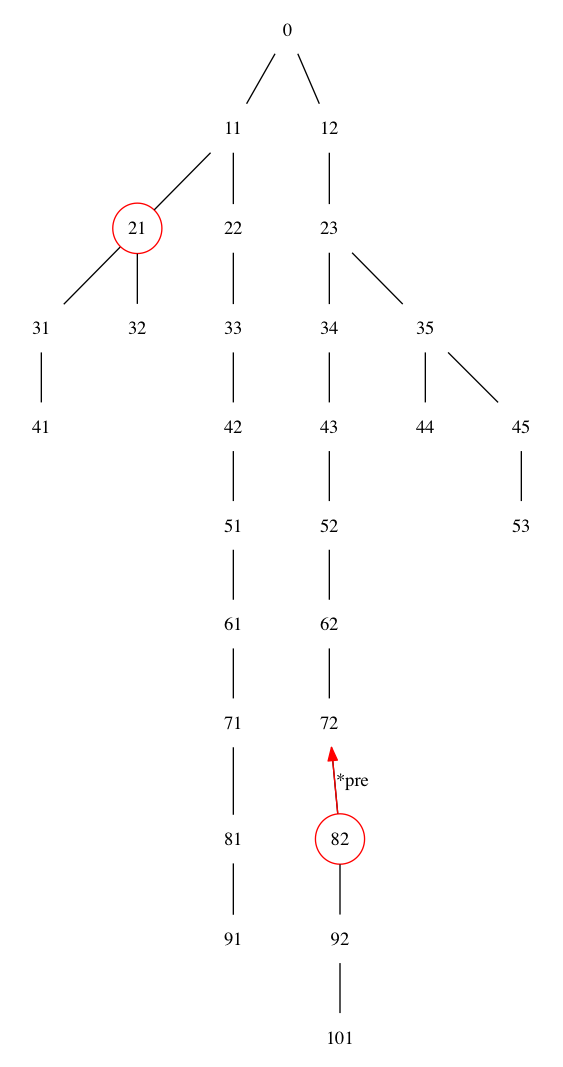
\includegraphics[scale=0.2]{tree.png}
}
\subfloat[$k^{1}$ tree]{
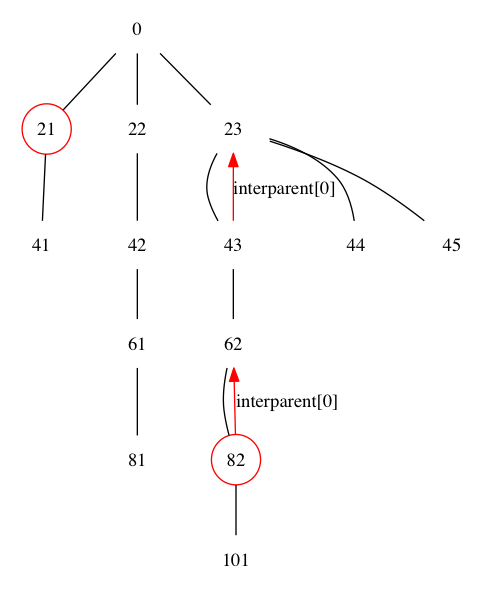
\includegraphics[scale=0.3]{tree1.png}
}
\subfloat[$k^{2}$ tree]{
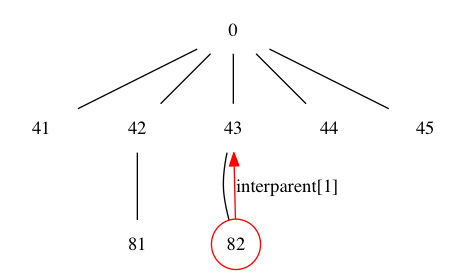
\includegraphics[scale=0.3]{tree2.png}
}
\label{fig:example}
\caption{Trees with k=2}
\end{figure}

\subsubsection{Checking conflict between two events in the same tree}
Tree are divided into layers whose events have the same depth and are in immediate conflict.
e and e' are two events in that tree at depths $e.depth$ and $e'.depth$ respectively.
\begin{itemize}
\item
	If $e.depth = e'.depth$, then $e \icfl e'$
\item
	If $e.depth \neq e'.depth$, without loss of any generality, assume $ depth(e) > depth(e')$ . Find an event $e": e" < e$ and $e".depth = e'.depth$ . If $e" \equiv e'$, then $e'$ and $e$ are in causality, else they are in conflict.
\end{itemize}

	
To quickly find $e"$ through the tree, we use the idea of skip list
(see \ref{fig:example}).
Accordingly, in each node, a list of skip predecessors $
skip\_preds = (i_1, i_2,..,i_m)$ are stored, where $i_j$ $(j \in [1,m] )$ is the
node's predecessor in $k^{j}$ distance of depth, k (k > 1) is a constant
distance in depth choosen to skip.\\

\noindent
\textbf{Data structure:}
Using template struct \verb!Node<T>:!
\begin{itemize}
	\item \textit{depth}: the distance from the root
	\item \textit{*pre}: according to the type of tree, it points to node of T which is immediate predecessor (\verb!pre-proc! or \verb!pre_mem! in Event class)
	\item \textit{skip\_preds}: list of pointers to its k-skip predecessors of type T.	
(T can be an event in the same process or touching the same variable)
\end{itemize}

To apply the algorithm of skip list to layered trees, we use a template class \verb!MultiNode<T>! (T is Event) which has the following attributes:
\begin{itemize}
	\item list of two \verb!Node! (first one for process, second one for variable)
	\item a template function $pred()$ to locate the predecessor corresponding to type of \verb!Node!
\end{itemize}
 
 Class Event inherits \verb!MultiNode<T>! and has two template function indicating which type of Node to take into account.
\begin{itemize}
\item	
	\verb!Node<Event> &proc!: return node in equivalant \textit{process} tree
\item	
	\verb!Node<Event> &var!: return node in equivalant \textit{variable} tree 	
\end{itemize}

\noindent
\textbf{Initialize a list of skip predecessors} \verb!skip_preds:!
\begin{itemize}
\item
	Firstly, we need to define the size $s$ of vector \verb!skip_preds! of a node. It depends on the depth of the node.

	 $s = max(i \in [1,\infty]: e.depth \mod k^{i} = 0 )$ 
\item
	Next, compute the entire list of skip predecessors for e. For every node, $e.skip\_preds[i]$ is a predecessor which is in a depth 			distance of $k^{i}$ with e, so that:
	\begin{itemize}
	\item
		The first element of the list \verb!skip_preds[0]! indicates the predecessor which is in a depth distance of $k^1 = k$. It can 				be reached by backtracking with $pre$ which is actually \verb!pre_proc! or \verb!pre_mem! of corresponding event.
	\item
		For $\forall i \in [1,s]: skip\_preds[i] = max(\{e": e" < e$ and $e".depth \mod k^i = 0\})$ which can be computed by going back 			k times with $skip\_preds[i-1]$: \\
		 \verb!e.skip_preds[i] = e.skip_preds[i-1]....skip_preds[i-1]! (k times) 
	\end{itemize}
\end{itemize}

\begin{algorithm}
\noindent
Assume $e.depth > e'.depth$, and , to reach e', do as follows:
\begin{enumerate}
\item
	\verb!Set next = e!
\item
	\verb!while! $next.depth \neq e'.depth$ \verb!do!
	\begin{itemize}
	\item
		\verb!Set d  = next.depth - e'.depth!
	\item
		\verb!Set i  = 0!
	\item
		\verb!while! ($ next.depth \mod k^{i} = 0$)   \space \verb!do!
		    $i = i + 1$
	\item
		\verb!Set! $next = next.skip\_preds[i]$ 
 	\end{itemize} 
\item 
	If $next \equiv e'$ then 
		$e'< e$ 
	
	else $e'\cfl e$	 
\end{enumerate}
\caption{Decide the conflict between e and e' in the same tree}
\label{a:layer_tree}	
\end{algorithm}

\begin{algorithm}
Given two reads $e$ and $e'$.
\begin{enumerate}
	\item
		Set \verb!w1 = e.find_WR_pred() !
			\verb!w2 = e'.find_WR_pred()!
	\item
		If $w_1 == w_2$
			return false;
	\item
		If $w_1 \cfl w_2$
			return true;
	\item
		If $w_2$ is a successor of $w_1$
		\begin{itemize}
			\item
				Set $w'$ is WR predecessor of $w_2$ at the $w_1.depth + 1$
			\item
				Set $r_1$ = \verb!w'.pre_preaders[e->trans->proc.id]!
			\item
				If ($e$ < $r_1$) then $\lnot (e \cfl e')$
				
				else 	$e \cfl e'$;
		\end{itemize}
		else
		\begin{itemize}
			\item
				Set $w'$ is WR predecessor of $w_1$ at the $w_2.depth + 1$
			\item
				Set $r_1$ = \verb!w'.pre_preaders[e'->trans->proc.id]!
			\item
				If ($e'$ < $r_1$) then $\lnot (e \cfl e')$
				
				else 	$e \cfl e'$;
		\end{itemize}
		
\end{enumerate}
\caption{Decide the conflict between two RDs}
\label{a:rds}	
\end{algorithm}

\begin{algorithm}
Given two events $e$ is a WR and $e'$ is a RD
\begin{enumerate}
	\item
		Set 	\verb!w2 = e'.find_WR_pred()!
	\item
		If $e == w_2$
			return false;
	\item
		If $e \cfl w_2$
			return true;
	\item
		If $w_2$ is a successor of $e$
		then $e < e'$
		else
		\begin{itemize}
			\item
				Set $w'$ is WR predecessor at the $w_2.depth + 1$
			\item
				Set $r_1 = w'.pre\_preaders[e'->trans->proc.id]$
			\item
				If ($e'$ precedes $r_1$) then $\lnot (e \cfl e')$
				
				else 	$e \cfl e'$;
		\end{itemize}
		
\end{enumerate}
\caption{Decide the conflict between a WR and a RD}
\label{a:wrd}	
\end{algorithm}

\begin{algorithm}
Given two events touching different variables or 2 LOCs $e$ and $e'$.
Do the following:
\begin{enumerate}
	\item
		For each pair $(e_i, e_i')$ of maximal events of each process:
		$e_i \in$ \verb!e.proc_maxevt! and $e_i' \in$ \verb!e'.proc_maxevt! do: \\
		\begin{itemize}
			\item
				If $e_i$.\verb!check_conflict_same_tree(!$e_i'$ \verb!)! is $true$, then  return true;
			\item
				Else jump to 2
		\end{itemize}
			
	\item
		For each pair $(e_i, e_i')$ of maximal events of each process:
		$e_i \in $ \verb!e.var_maxevt! and $e_i' \in$ \verb!e'.var_maxevt! do:\\
			\begin{itemize}
			\item
				If $e_i$.\verb!check_conflict_same_tree(!$e_i'$ \verb!)! is $true$, then  return true;
			\item
				Else, return false;
		\end{itemize}
			
\end{enumerate}
\caption{Decide the conflict between 2 LOCs}
\label{a:arb}	
\end{algorithm}


\section{Exloration algorithm}
\begin{algorithm}
Let C is current configuration, D is a set of disable events, A is a set of events to be added.

At the beginning, set $C = \{\bot \}$, $D = \emptyset$, $A = \emptyset$ 
\begin{enumerate}
	\item
		Compute C.en and C.cex at the state of C
	\item
		If $C.en = \emptyset$, then return
	\item
		Else 
		\begin{itemize}
			\item
				If ($A = \emptyset$), then take the event $e$ at the back of C.en
				(Remember to pop up the event from C.en)
			\item
				else take $e$ satisfying: $e \in A$ and $e \in C.en$
				(Remember to pop up the event from both A and C.en))
		\end{itemize}
	\item
		Store current configuration for alternative computing function
	\item
		C.add(e) 
	\item
		Call Explore(C,D,A)
	\item
		Remove the last added event from C to D: 
		\begin{itemize}
		\item
			\verb!C.remove(e)! (retrieve the previous configuration)
		\item
			\verb!D.push_back(e)!
		\end{itemize}
	\item
		$J = compute\_alt(C,D)$
		\begin{itemize}
			\item
				If J is not empty, then
				\begin{itemize}
					\item
						update $A = \{e: e \in J$ and $e\not\in C\}$
					\item
						Call Explore(C,D,A)
				\end{itemize}
			\item
				If J is empty, then backtrack to the previous C
		\end{itemize}
	\item
		$D.pop\_back()$
\end{enumerate}

\caption{Unfolding based POR exploration algorithm}
\label{a:exp}	
\end{algorithm}

%Algorithm to find out all alternatives

\begin{algorithm}
\noindent
Remove from D all events in cex(C).
For each event $e_i \in D$, repeat the following:
\begin{enumerate}
\item
	Let $comb \eqdef \tup{s_1, \ldots, s_n}$ be the comb over A . 
	$s_i$ are the events in direct conflict to $e_i$: $s_i$ = $e_i$ \verb!->dicfl!
\item
	Remove from the $comb$ all events that are in conflict with any maximal event of C
\item
	Enumerate all combinations $\tup{e_1, \ldots, e_n}$ of $c$.
\item
	For any of them, do:
	\begin{itemize}
		\item 
    		If $\tup{e_1, \ldots, e_n}$ is conflict-free, return $J = \cup e_i$ 
   		\item
			If there exist any conflict among events in J, then discard J and come back to step 2
			to take next combination.
	\end{itemize}
\item End.
\end{enumerate}
\caption{Computing an alternative J for D after C}
\label{a:alter}
\end{algorithm}


\section{LLVM Frontend}

\subsection*{Pass 1: Sanity Checks}

Conditions to accept the input LLVM program:

\begin{itemize}
\item
  \verb!pthread_create! must be called directly from the main function and not
  in a loop or within a conditional.
\item
  \verb!printf!,
  \verb!pthread_{create,join,mutex_lock,mutex_unlock}! are the only function calls
  allowed (\verb!create! only in main).
\item
  All \verb!alloca! must be found in the first \verb!BasicBlock! of the
  function, and no block can jump into that block (not in a loop).
\item
  All variables in the C program are integers or arrays integers.
\end{itemize}

\subsection*{Pass 2: Construction of 3-address IR}

\subsection*{Pass 2.1: Identification of Threads}

\begin{itemize}
\item Number of threads given on command line
\item Finding out the C function executed by each thread
\end{itemize}

\subsection*{Pass 2.3: Allocation of memory}

\begin{itemize}
\item
  For each global symbol (\verb!@sym!), allocated memory space (\verb!alloca!
  instruction), and local register (\verb!%sym!) we allocate space in the
  memory of our virtual machine
\item
  We generate a symbol table mapping each address to a textual name.
\end{itemize}

\subsection*{Pass 2.4: Translation to 3-address IR}

Textual format and translation of LLVM opcodes in
\verb!doc/internals/3addr-ir.rst!.

\subsection*{Pass 2.5: Reduction of target variables based on live variable
analysis}

Only if we have time, although this could be done based on LLVM information and
directly during the translation of LLVM instructions to ou 3-address code.

\url{https://en.wikipedia.org/wiki/Live_variable_analysis}

\subsection*{Pass 3: Construction of Large-Block Encoding}

\subsection*{Pass 3.1: Identification of local and global variables}
\begin{itemize}
\item
  For us a variable is a 4 bytes block or an 8 bytes block, starting at an
  address multiple of, respectively, 4 or 8 bytes. Any memory access should
  regard exactly the 4 or 8 bytes inside a variable or any byte or 2 bytes inside a
  variable, but should never involve bytes belonging to two variables.
  Make a pass that ensures this for directy memory access instructions, for
  indirect accesses we will pray (think of this in the future).
\item
  A symbol (pair address-size $\tup{a,s} \in \N \times \N$) is \emph{local} to a
  thread if that thread is the only one that can modify the addresses
  $a, a+1, a+2, \ldots, a+s-1$.
  It is \emph{global} if it is not local.
  Make a pass to detect the variables local to each thread and the global ones.
\item
  We assume that one thread will never pass a pointer to some of its local
  variables or arrays to the other thread. On a later stage we will implement a
  points-to static analysis to detect this.
  So for now we ingore the \verb!movid! and \verb!movis! instructions.
\end{itemize}

\subsection*{Pass 3.2: Instruction splitting: 0 or 1 global access per instruction}

Rewrite instructions that make use of 2 or 3 global addresses to make use of at
most 1 global variable.
Use auxiliary local variables to store intermediate values. Easy.

For \verb!movis!, \verb!movid!, \verb!brz!, and \verb!brnz! instructions,
rewrite them so they use 0 global addresses.

\subsection*{Pass 3.3: Construction of large blocks}

An indirect instruction is either \verb!movid! or \verb!movis!.
A local instruction is one that only refers to local addresses and is not
indirect.
A branch instruction is either
\verb!brz! or \verb!brnz! (by assumption branch instructions are local).
A global instruction is one that is not local or indirect.

The first block of a thread is composed of all instructions of the first basic
block that are local and not branch.

All remaining blocks start at a
\begin{itemize}
\item branch instructions,
\item indirect instruction, or
\item global instruction.
\end{itemize}

\section{FIXMEs}

- do we need \verb!post_*! in any event? -> necessary for check shared parents among events

- do we need \verb!pre_mem! in \verb!WR! events? -> Yes, for WR tree in conflcit checking

\newpage

\bibliography{refs}
\bibliographystyle{splncs}


\end{document}

